\section{Christoffer}
% \begin{frame}{Christoffer}
% \begin{itemize}
%   \only<1->{\item This}
%   \only<2->{\item is}
%   \only<3->{\item a}
%   \only<4>{\item test}
% \end{itemize}
% \end{frame}

\begin{frame}{Christoffer}
\begin{itemize}
  \item The tasks of our program
  		\begin{enumerate}
  			\item What is each tasks purpose
  			\item Key implementation points of each task
  			\item Why they are implemented as they are  
		\end{enumerate}
  \item Unit tests
  		\begin{enumerate}
  			\item How have we unit tested
  			\item The framework
  			\item The results of the test
		\end{enumerate}
  \item The final test of the turret
%   		\begin{enumerate}
%   			\item 
% 		\end{enumerate}
\end{itemize}
\end{frame}

\subsection{Tasks}
\begin{frame}{Tasks}
\begin{itemize}
  \item Main
  \item Track
  \item GetDataAndCalculate
  \item WaitAndFire
\end{itemize}
\end{frame}

\begin{frame}[fragile]{Main}
\only<1-3>{
\begin{itemize}
  \item Purpose
  	\only<2>{
  	\begin{itemize}
  		\item Start tasks
  		\item Setup
  	\end{itemize}
  	}
  \only<3>{\item Key implementation points}
\end{itemize}
}
\begin{onlyenv}<4>
\begin{center}
\begin{minipage}[H]{0.9\linewidth}
\begin{lstlisting}
PosRegEnable(ROTATE_MOTOR);
PosRegEnable(ANGLE_MOTOR);
SetMotorRegulationTime(10);
NXTCam_Init(CAM_PORT, CAM_ADDR);
NXTCam_SendCommand(CAM_PORT, CAM_ADDR, 'A'); 
NXTCam_SendCommand(CAM_PORT, CAM_ADDR, 'E');
SetSensorUltrasonic(SENSOR_LEFT);
SetSensorUltrasonic(SENSOR_RIGHT);
Precedes(Track,GetDataAndCalculate);
\end{lstlisting} 
\end{minipage}
\end{center}
\end{onlyenv}
\end{frame}

\begin{frame}[fragile]{Track}
\only<1-3>{
\begin{itemize}
  \item Purpose
  	\only<2>{
  	\begin{itemize}
  		\item Track targets
  		\item Information sharing
  	\end{itemize}
  	}
  \only<3>{\item Key implementation points}
\end{itemize}
}
\begin{onlyenv}<4>
\begin{center}
\begin{minipage}[H]{0.9\linewidth}
\begin{lstlisting}
while(track){
	NXTCam_GetBlobs(CAM_PORT, CAM_ADDR, nblobs, bc, bl, bt, br, bb);
    if(nblobs > 0){
    	blobInCam = true;
        ....
        if(lib_direction != NO_DIRECTION){
        	tempSpeed = GetSpeed(blobCenter );
            if(tempSpeed > 0 && lib_direction == RIGHT_DIRECTION)
            	OnFwd(ROTATE_MOTOR, tempSpeed);
            else if(tempSpeed < 0 && lib_direction == LEFT_DIRECTION)
            	OnFwd(ROTATE_MOTOR, tempSpeed);
        }
	}else{
    	blobInCam = false;
        ...
    	Off(ROTATE_MOTOR);
	}
    DetermineDirection(blobCenter, oldBlobCenter, directionCount);
}
\end{lstlisting} 
\end{minipage}
\end{center}
\end{onlyenv}
\end{frame}

\begin{frame}[fragile]{GetDataAndCalculate}
\only<1-3>{
\begin{itemize}
  \item Purpose
  	\only<2>{
  	\begin{itemize}
  		\item Collect data
  		\item Calculate vectors and positions
  		\item Determine the shooting position
  	\end{itemize}
  	}
  \only<3>{\item Key implementation points}
\end{itemize}
}
\begin{onlyenv}<4>
\begin{center}
\begin{minipage}[H]{0.9\linewidth}
\begin{lstlisting}
while(collecting){
	if(blobInCam){
        if(length != NO_DATA){
            if(MakePosData(length,GetMotorAngle(),CurrentTick(),tempPosData)){
            	posData[posDataCounter] = tempPosData;
                posDataCounter++;
            }
            if(posDataCounter == DATASETS_NEEDED_TO_CALCULATE){
				track = false;
                Off(ROTATE_MOTOR); 
                StopTask(Track);
                DirectionVector vector = CalcDirVector(posData,posDataCounter);
                fire = CalcFireData(CalcFuturePos(vector,MILLISECONDS_TO_HIT));
                StartTask(WaitAndFire);
            }
    	}
	}
}
\end{lstlisting} 
\end{minipage}
\end{center}
\end{onlyenv}
\end{frame}

\begin{frame}[fragile]{WaitAndFire}
\only<1-3>{
\begin{itemize}
  \item Purpose
  	\only<2>{
  	\begin{itemize}
  		\item Wait until the calculated time
  		\item Shoot the target at the calculated position
  		\item Reset the turret
  	\end{itemize}
  	}
  \only<3>{\item Key implementation points}
\end{itemize}
}
\begin{onlyenv}<4>
\begin{center}
\begin{minipage}[H]{0.9\linewidth}
\begin{lstlisting}
collecting = false;
LoadRound();
Off(ROTATE_MOTOR);
RotateH(fire.angleH);
Angle(fire.angleV);
while(true){
	if(CurrentTick() >= fire.timeToHit && !alreadyFired){
    	alreadyFired = true;
        Fire();
        break;
    }
}
Angle(START_ANGLE);
...
Wait(4000);
StartTask(Track);
StartTask(GetDataAndCalculate);
\end{lstlisting} 
\end{minipage}
\end{center}
\end{onlyenv}
\end{frame}

\subsection{Unit Test}
\begin{frame}[fragile]{Unit Test}
\begin{itemize}
  \only<1-2,6-8>{\item How have we tested}
  \only<2-2,6-8>{\item No framework}
  \only<6-8>{\item What have we tested}
  			\only<7>{
  			\begin{enumerate}
  				\item CalcDirVector
  				\item UpperBound
  				\item CheckLength
  				\item GetSpeed
  				\item And more\ldots
  			\end{enumerate}
  			}
  \only<8-9>{\item Results} 
\end{itemize}
\begin{onlyenv}<3>
\begin{center}
\begin{minipage}[H]{0.9\linewidth}
\begin{lstlisting}
bool CombineVectorsTest2(){
	DirectionVector input1;
	input1.speedX = 10;
  	input1.speedY = 10;
  	input1.xPos = 15;
  	input1.yPos = 15;

  	DirectionVector dirVecArray[1];
  	dirVecArray[0] = input1;
  	DirectionVector out = CombineVectors(dirVecArray, 1);

  	if(out.speedX == 10 && out.speedY == 10 && out.xPos == 15, out.yPos == 15){
    	return true;
  	}
  	else {
    	return false;
  	}
}

bool UpperBoundTest(int input, int expected){
	int out = UpperBound(input);

  	return Assert(out, expected);
}
\end{lstlisting} 
\end{minipage}
\end{center}
\end{onlyenv}
\begin{onlyenv}<4>
\begin{center}
\begin{minipage}[H]{0.9\linewidth}
\begin{lstlisting}
task main(){
	unsigned int rtn_code = CreateFile(NAME, SIZE, handle);
   	if (rtn_code == LDR_FILEEXISTS)
     	rtn_code = OpenFileAppend(NAME, SIZE, handle);
  	...
 	if(UpperBoundTest(130, 130)){
    	WriteLn(handle, "UpperBoundTest: Passed");
  	}
 	else{
    	WriteLn(handle, "UpperBoundTest: Failed");
  	}
  	if(UpperBoundTest(240, 144)){
    	WriteLn(handle, "UpperBoundTest2: Passed");
  	}
  	else{
    	WriteLn(handle, "UpperBoundTest2: Failed");
  	}
  	if(CombineVectorsTest2()){
    	WriteLn(handle, "CombineVectorsTest2: Passed");
  	}
  	else{
    	WriteLn(handle, "CombineVectorsTest2: Failed");
  	}
  	...
  	CloseFile(handle);
}
\end{lstlisting} 
\end{minipage}
\end{center}
\end{onlyenv}

\begin{onlyenv}<5>
\begin{itemize}
  \item How have we tested
  \item No framework
  \begin{itemize}
  \item Non testable function
\end{itemize}
\end{itemize}
\begin{center}
\begin{minipage}[H]{0.9\linewidth}
\begin{lstlisting}
float GetMotorAngle(){
    return MotorRotationCount(ROTATE_MOTOR)*0.73;
}
\end{lstlisting} 
\end{minipage}
\end{center}
\end{onlyenv}
\only<9>{
\begin{figure}[H]
  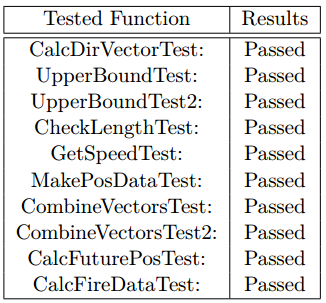
\includegraphics[scale=0.5]{figures/result.png}
\end{figure}
}
\end{frame}

\subsection{Final Test}
\begin{frame}{Final Test}
\begin{itemize}
  \only<1-4>{\item Setup}
  \only<2-4>{\item Execution}
  \only<3-4>{\item Observations}
  \only<4->{\item Result}
  \only<5>{
\begin{figure}[H]
  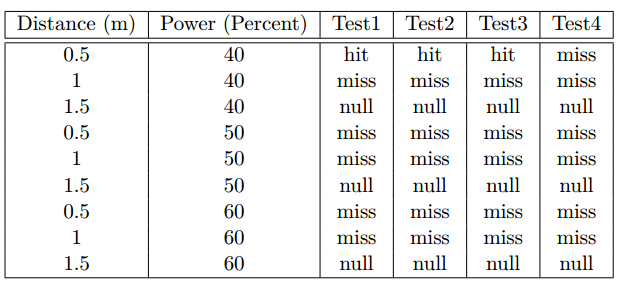
\includegraphics[scale=0.5]{figures/finalTestResult.png}
\end{figure}
}
\end{itemize}
\end{frame}